\documentclass{beamer}

\usepackage[utf8]{inputenc}
\usepackage{booktabs}
\usepackage{xcolor}
%\usetheme{Hannover}
\usecolortheme{crane}
\usepackage{siunitx,cancel}
\usepackage{graphicx}
\usepackage{hyperref}

\usepackage{listings}
\usepackage{color}
\usepackage{xcolor}

%\usepackage[
%backend=biber,
%style=numeric,
%citestyle=numeric,
%sorting=none
%]{biblatex}
%\addbibresource{resources.bib}


% This is the color used for MATLAB comments below
\definecolor{MyDarkGreen}{rgb}{0.0,0.4,0.0}
\definecolor{Blue}{rgb}{0.0,0.0,1.0}
\definecolor{Purple}{rgb}{1.0,0.0,1.0}

\colorlet{mygray}{black!30}
\colorlet{mygreen}{green!60!blue}
\colorlet{mymauve}{red!60!blue}

\lstset{
  backgroundcolor=\color{gray!10},
  basicstyle=\ttfamily,
  columns=fullflexible,
  breakatwhitespace=false,
  breaklines=true,
  captionpos=b,
  commentstyle=\color{mygreen},
  extendedchars=true,
  frame=single,
  keepspaces=true,
  keywordstyle=\color{blue},
  language=c++,
  numbers=none,
  numbersep=5pt,
  numberstyle=\tiny\color{blue},
  rulecolor=\color{mygray},
  showspaces=false,
  showtabs=false,
  stepnumber=5,
  stringstyle=\color{mymauve},
  tabsize=3,
  title=\lstname
}






%\defaultfontfeatures{Scale=MatchLowercase,Mapping=tex-text}
%\setmainfont[Numbers=Lowercase]{Minion Pro}
%\setsansfont[Numbers=Lowercase]{Myriad Pro}
%\setmonofont{Menlo}
%\setmathsfont(Digits,Latin,Greek)[Numbers={Lining,Proportional}]{Minion Pro}

\sisetup{%
  output-decimal-marker = {.},
  per-mode = symbol,
  %round-mode = places,
  %round-precision = 5
}

\DeclareSIUnit \electronvolt {\ensuremath{eV}}
\DeclareSIUnit \lightspeed {\ensuremath{c}}
\DeclareSIUnit \dalton{\ensuremath{u}}
\DeclareSIUnit \echarge{\ensuremath{e}}


\newcommand{\mvec}[2]{
\ensuremath{\left(
\begin{array}{c}
#1\\
#2\\
\end{array}
\right)}
}

\newcommand{\Span}{\ensuremath{\mathrm{Span}}}
\newcommand{\Mat}{\ensuremath{\mathrm{Mat}}}
\newcommand{\R}{\ensuremath{\mathbb{R}}}
\newcommand{\Rno}{\ensuremath{\mathbb{R}\backslash\{0\}}}
\newcommand{\Z}{\ensuremath{\mathbb{Z}}}
\newcommand{\ol}[1]{\ensuremath{\overline{#1} } }
\newcommand{\F}[1]{\ensuremath{\mathbb{F}_{#1} } }


%Information to be included in the title page:
\title{MAINTITLE}
\author{Nikolaj Roager Christensen}
\institute{Student Colloquium in Physics and Astronomy, Aarhus University}
\date{March 2021}

%\AtBeginSection[]
%{
%}

\titlegraphic
{
TITLEIMAGE
%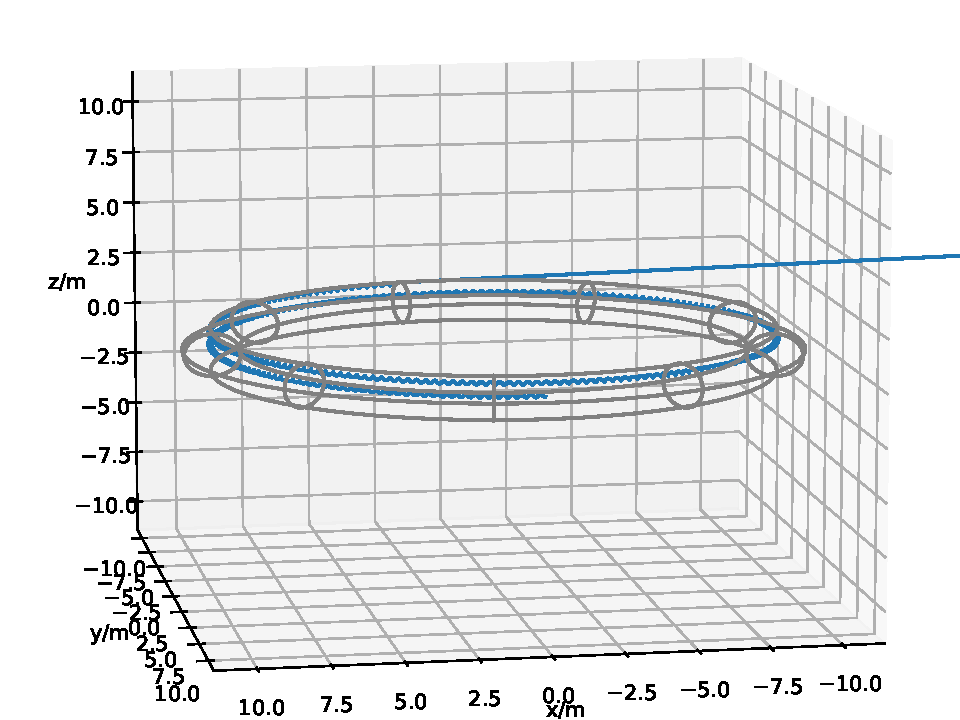
\includegraphics[width=0.5\textwidth]{torus4_3D.pdf}
}
\begin{document}

\frame{\titlepage}



\section{Introduction [3 MIN]}

\begin{frame}
\frametitle{MAINTITLE}
\tableofcontents
\end{frame}


\begin{frame}
\frametitle{Introduction, what and why}
\begin{columns}
\begin{column}{0.5\linewidth}
\begin{itemize}
\item<1->
\begin{itemize}
\item<3->
\end{itemize}
\end{itemize}
\end{column}
\begin{column}{0.5\linewidth}

%\only<2>
%{%
%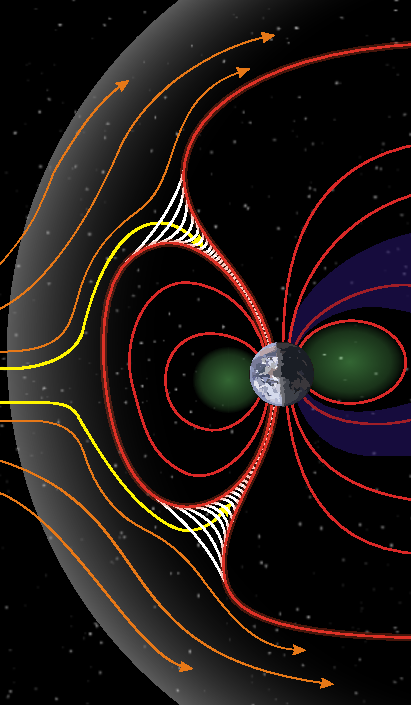
\includegraphics[width=0.8\linewidth]{Structure_of_the_magnetosphere_Nasa.pdf}%
%{\color{gray} Illustration originally from Nasa. Published on wikipedia, in Public Domain (Cropped to fit page) }
%}%
\end{column}
\end{columns}
\end{frame}


\begin{frame}
\frametitle{How: Numeric-ODE solvers}
\begin{itemize}
\item<1-> When analytical solutions are not practical.
\item<2-> Testing experimental setups.
%\item<4-> Here, the \lstinline{odeint} library in C++.
%\begin{itemize}
%\item<4-> Runge Kutta Algorithm
%\item<4-> Identical to \lstinline{odeint}/\lstinline{ode45} in scipy or matlab.
%\end{itemize}
\item<5-> Simulations are not experiments!
\end{itemize}
\end{frame}


\section{Theory and physical background [10 MIN]}

\begin{frame}
\frametitle{Theory: Classical non-relativistic particles}
\begin{itemize}
\item<1-> Some repetition from Electrodynamics
\item<2-> The Lorentz force (SI units):

\begin{equation*}
\vec{F} = q ( \vec{v}\times \vec{B}+\vec{E}).
\end{equation*}

\item<3-> Only 1 particle! so pre-programmed depending on the setup.

\item<4-> Could use potentials $\phi(\vec{r},t)$ $\vec{A}(\vec{r},t)$ and Hamiltonian.
\end{itemize}
\end{frame}

\subsection{Solved systems}

\begin{frame}
\frametitle{Known results, cyclotron motion $\vec{B}$ fields}
\begin{columns}
\begin{column}{0.5\linewidth}
\begin{itemize}
\item<2-> Magnetic forces do no work:

\begin{equation*}
dW_{\vec{B}}= \vec{F}_B \cdot d\vec{r}\propto (\vec{v}\times \vec{B})\cdot \vec{v} = 0.
\end{equation*}

\item<3-> ($\vec{v}=\vec{v}_\perp+\vec{v}_\parallel$):

\begin{equation*}
|\vec{F}_B| = |q ( \vec{v}\times \vec{B})| =|q v_{\perp} B|.
\end{equation*}
\item<4-> Same as Centripetal force: Cyclotron motion

\item<5-> Cyclotron radius and frequency:

\begin{equation*}
R = \frac{v_\perp m}{|q|B} \quad \omega_c =\frac{|q|B}{m}.
\end{equation*}

\end{itemize}
\end{column}
\begin{column}{0.5\linewidth}
\only<1-2>{%
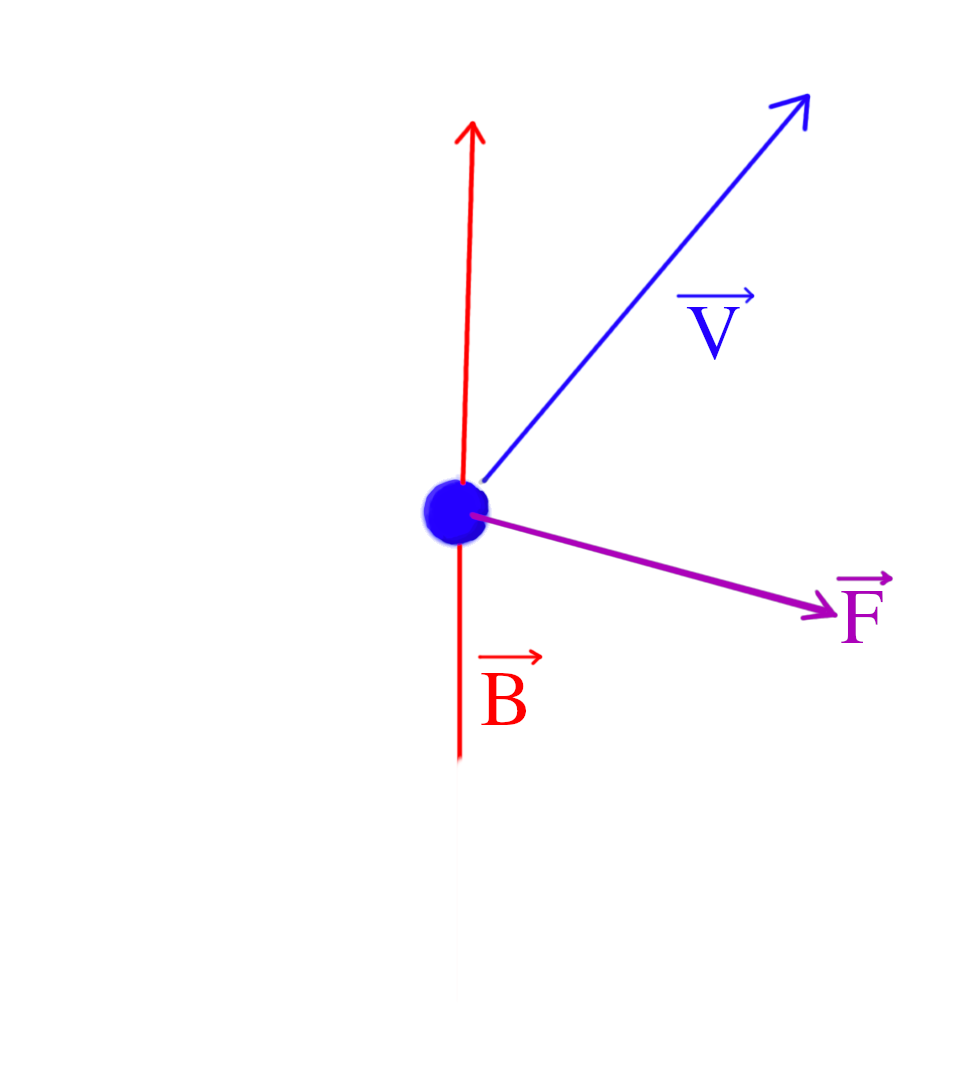
\includegraphics[width=\linewidth]{dw0.png}}%
\only<3->{%
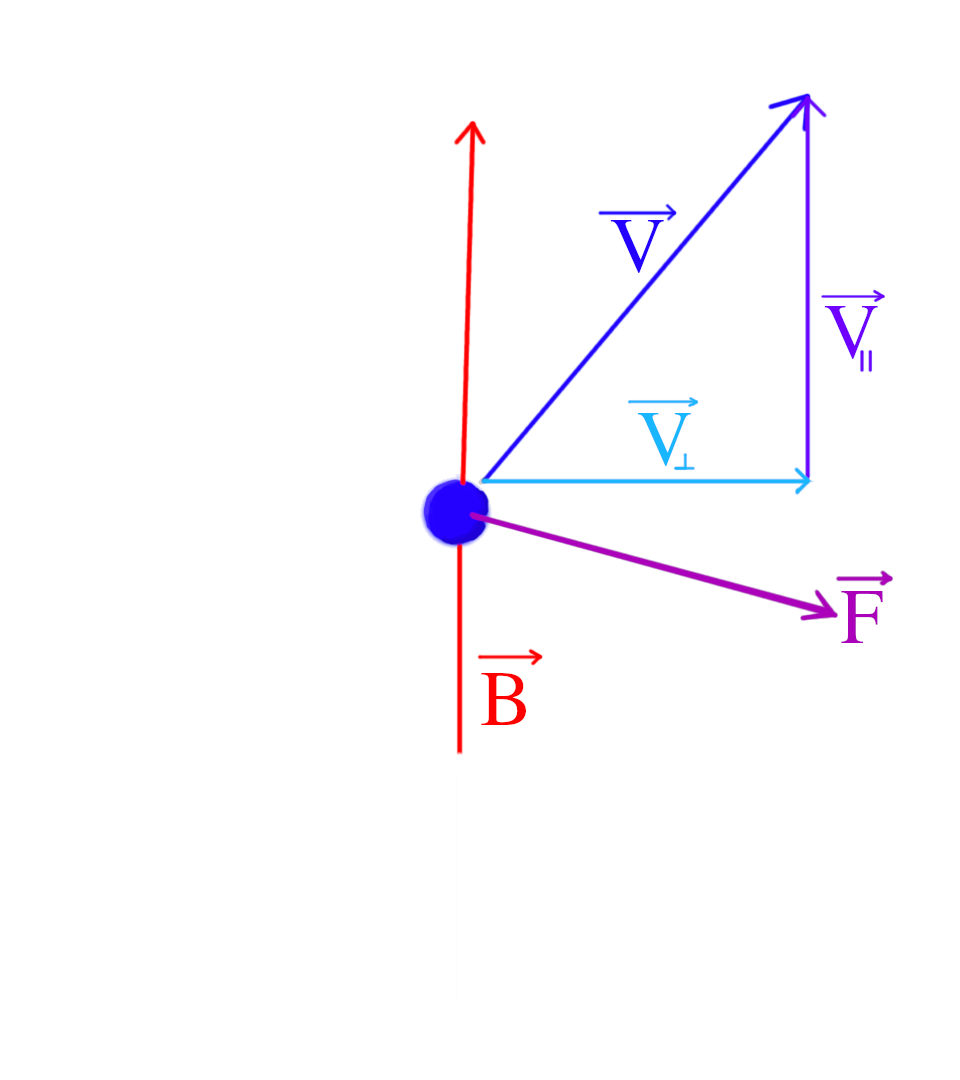
\includegraphics[width=\linewidth]{cyc0.png}}%
%\only<4->{%
%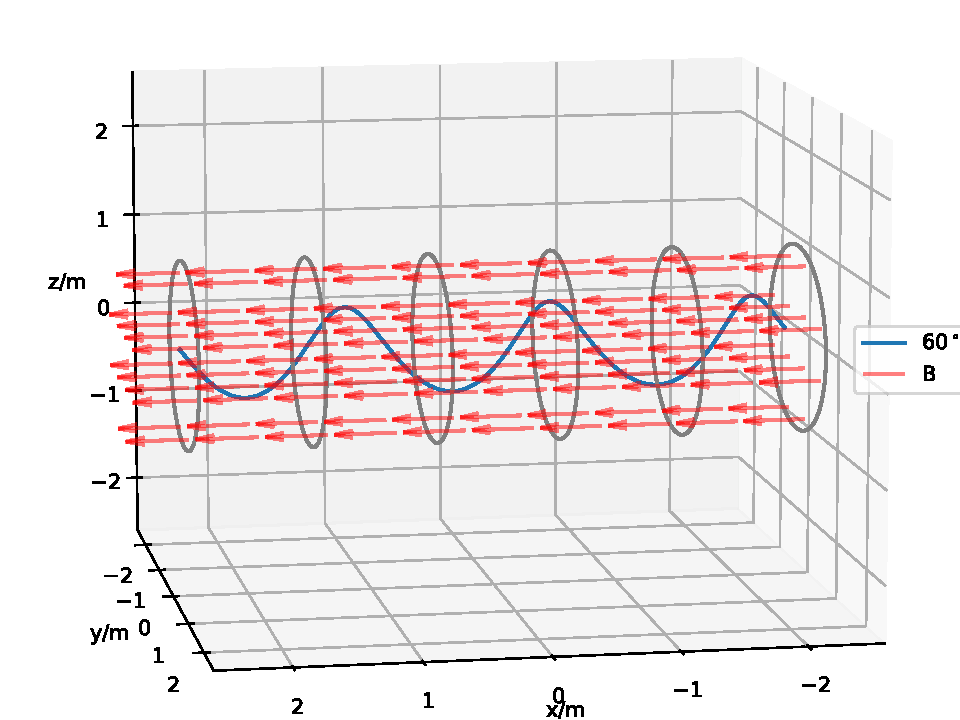
\includegraphics[width=\linewidth]{helix.pdf}}%
\end{column}
\end{columns}
\end{frame}

\begin{frame}
\frametitle{Analytical solution: Protons in a Solenoid}
\only<1>{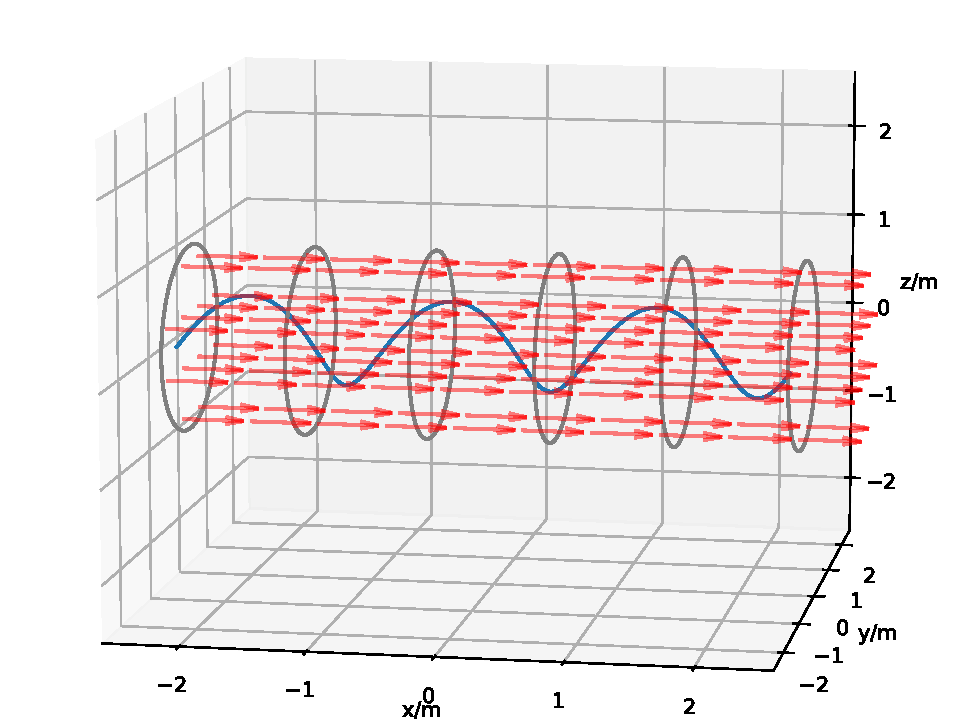
\includegraphics[width=0.8\linewidth]{AN_helix0.pdf}}%
\only<2>{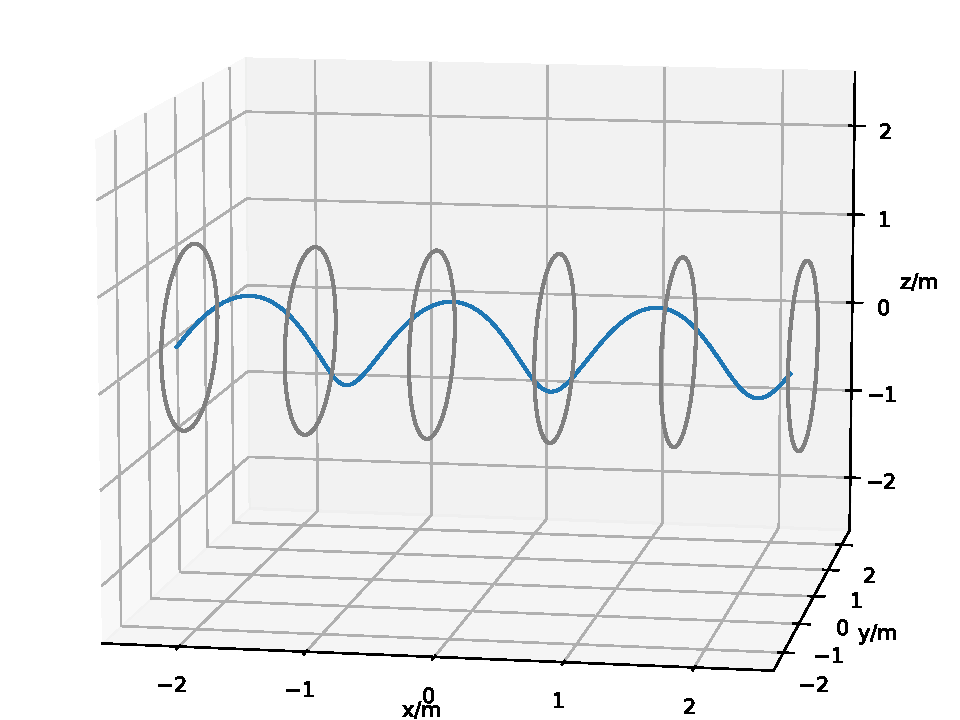
\includegraphics[width=0.8\linewidth]{AN_helix1.pdf}}%
\only<3>{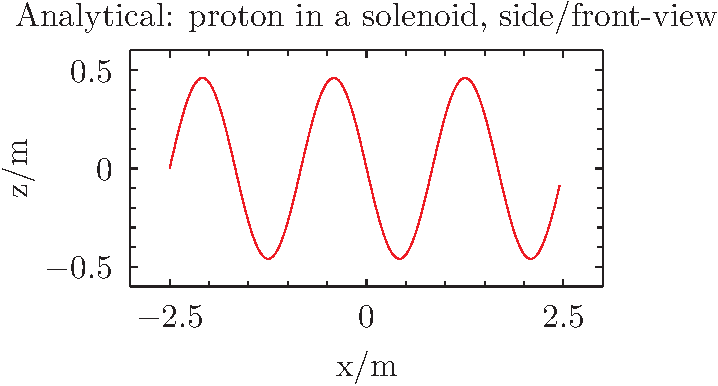
\includegraphics[width=0.66\linewidth]{AN_solenoid_xz_view.pdf}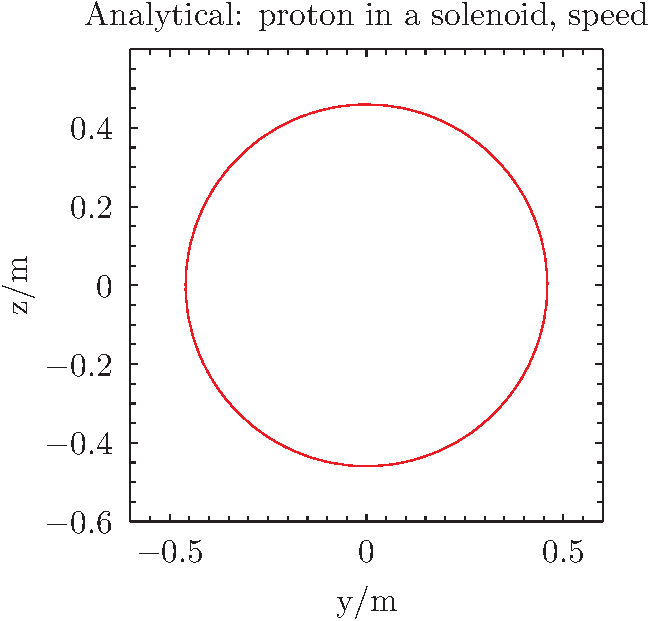
\includegraphics[width=0.33\linewidth]{AN_solenoid_yz_view.pdf}}%
\only<4>{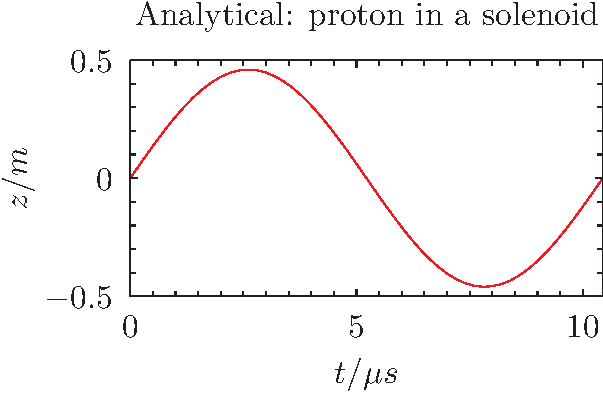
\includegraphics[width=\linewidth]{AN_solenoid_tz.pdf}}%
\only<5>{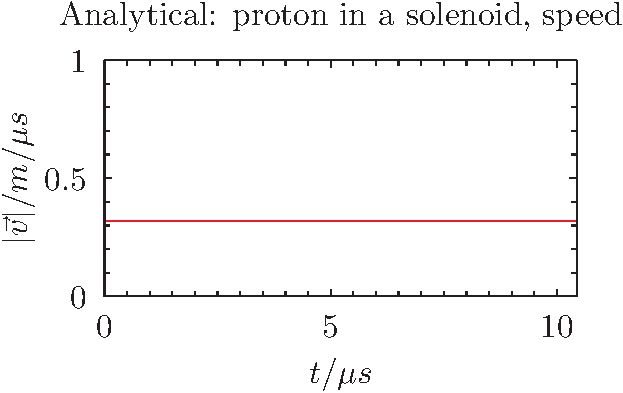
\includegraphics[width=\linewidth]{AN_solenoid_speed.pdf}}%

\only<1>{%
{\color{gray} Solenoid with $N=1000$ turns per $m$, $I=\SI{5}{\ampere}$, $r=\SI{1}{\meter}$, $|\vec{B}|\approx\SI{6}{\milli\tesla}$. Proton with $E_{kin}=\SI{1}{\mega\electronvolt\per\square\lightspeed}$ ($|v|\approx \SI{3.195E5}{\meter\per\second}$)}}
\only<2->{%
\begin{equation*}
R \approx \SI{0.5}{\meter}\sin(\theta) \quad T=\frac{2\pi}{\omega_c} \approx \SI{10}{\micro\second}
\end{equation*}
}
\end{frame}

\begin{frame}
\frametitle{Cyclotron accelerator}
\begin{columns}
\begin{column}{0.5\linewidth}
\begin{itemize}
\item<1-> Electric forces do work.

\item<2-> Practical example, the Cyclotron.

\item<3-> Single gab, oscillating field.

\item<4-> Final speed:

\begin{equation*}
\frac{R|q|B}{m} = v_\perp
\end{equation*}

\end{itemize}
\end{column}
\begin{column}{0.5\linewidth}
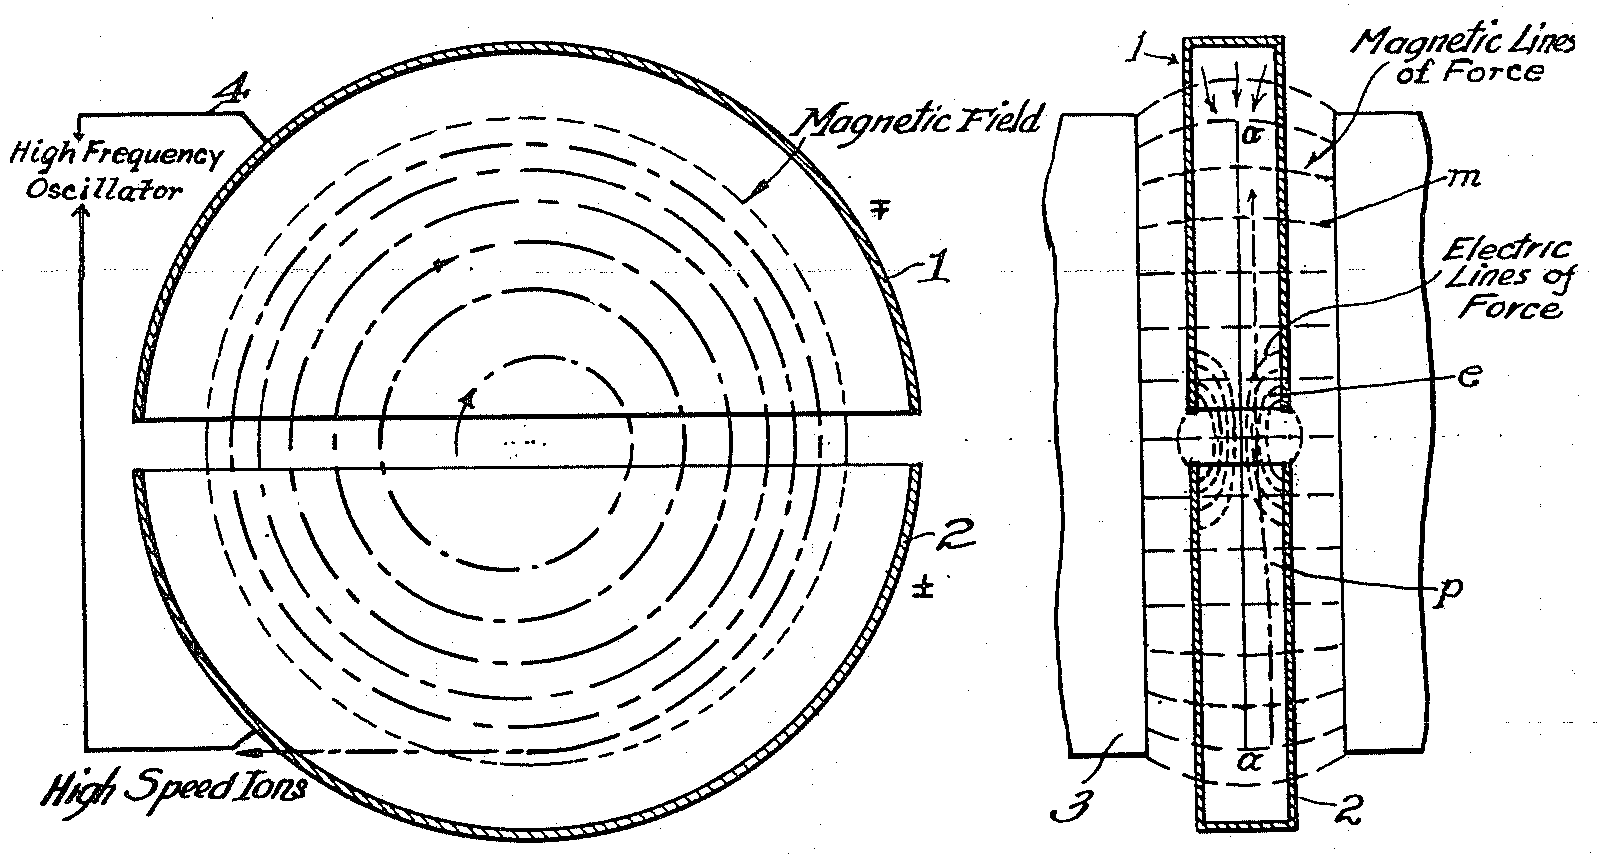
\includegraphics[width=\linewidth]{ Cyclotron_patent.png}
{\color{gray} Ernest O. Lawrence, 1934, U.S. Patent 1,948,384; image in Public Domain.}
\end{column}
\end{columns}
\end{frame}

\section{Eulers Method and the 4th order Runge-Kutta Method [10 MIN]}
%What are they, what are not they

\begin{frame}
\frametitle{Ordinary differential equation*s.}
\begin{itemize}
\item<1-> {\color{gray} Sources: Zeigler et al. Theory of Modeling and Simulation (Third edition) chapter 3}

\item<1-> Algorithms exists for ODEs:

\begin{equation*}
\dot{\mathbf{X}} = f_{ode}(\mathbf{X}(t),t).
\end{equation*}

\item<2-> We have a:

\begin{align*}
\ddot{\vec{r}} &= \frac{q}{m} ( \dot{\vec{r}}\times \vec{B}(\vec{r},t)+\vec{E}(\vec{r},t)).
\end{align*}

\item<3-> Here:

\begin{align*}
\mathbf{X} = \mvec{\vec{r}}{\dot{\vec{r}}} \quad f_{ode}(\vec{r},t) = \mvec{\dot{\vec{r}}}{\frac{q}{m} ( \dot{\vec{r}}\times \vec{B}(\vec{r},t)+\vec{E}(\vec{r},t))}.
\end{align*}
\end{itemize}
\end{frame}

\newif\ifadditional
%\additionalfalse
\additionaltrue

\ifadditional
\begin{frame}[fragile]
\frametitle{The ODE to solve}
%\only<1>{%
\begin{lstlisting}
auto ODE = [...](const state_type Data, state_type &dDatadt, const double t){
    //Extract position and velocity from data
    vec pos = vec(Data[0],Data[1],Data[2]);
    vec velocity = vec(Data[3],Data[4],Data[5]);

    //Lorentz+Newtons 2nd law
    vec F = Charge*(Fields.get_Efield(pos,t)+
        cross(velocity,Fields.get_Bfield(pos,t)));
    vec dVdt = F*Inv_mass;

    //Save derivative of data
    dDatadt[0]=velocity.x;
    ...
};
\end{lstlisting}
\end{frame}
\fi


\subsection{Euler's Method}

\begin{frame}
\begin{columns}
\begin{column}{0.5\linewidth}
\frametitle{The Forward Euler's Method}
\begin{itemize}
\item<1-> Let $h=t_{i+1}-t_i>0$ be constant.

\item<2-> $h$, $\mathbf{X}(t)$, $t_i$ and $f_{ode}$ are known.

\begin{equation*}
\dot{\mathbf{X}} = f_{ode}(\mathbf{X}(t),t).
\end{equation*}

\item<3-> How would you find $\mathbf{X}(t_{i+1})$:

\item<5-> \only<5,7>{(Explicit) Forward}\only<6>{(Implicit) Backward} Euler's Method:

\begin{equation*}
\mathbf{X}(t_{i+1}) = \mathbf{X}(t_{i})+h f_{ode}(\mathbf{X}(\only<5,7>{t_i}\only<6>{t_{i+1}}),t_i).
\end{equation*}


\item<1-> {\color{gray} Bernard P. Zeigler et al. Theory of Modeling and Simulation (Third edition), chapter 3}
\end{itemize}
\end{column}
\begin{column}{0.5\linewidth}
\only<1-3>{%
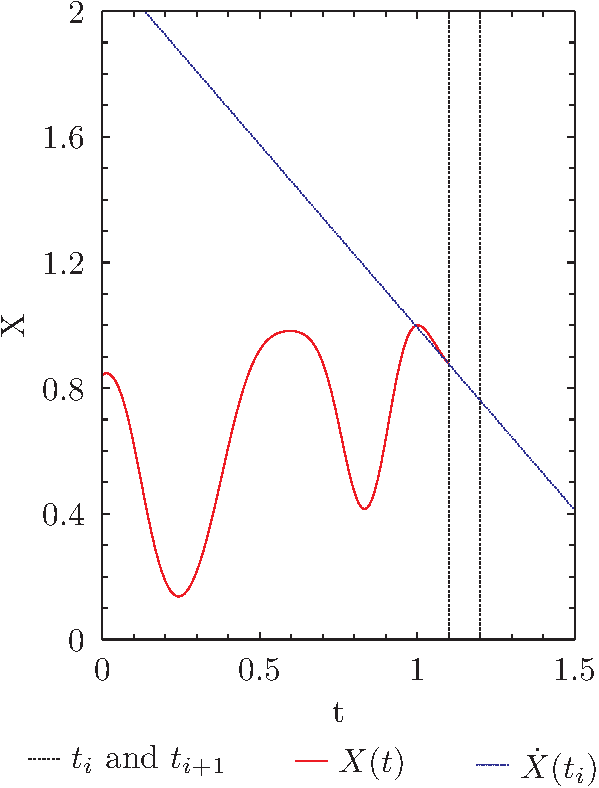
\includegraphics[width=\linewidth]{euler_demo0.pdf}%
}%
\only<4-6>{%
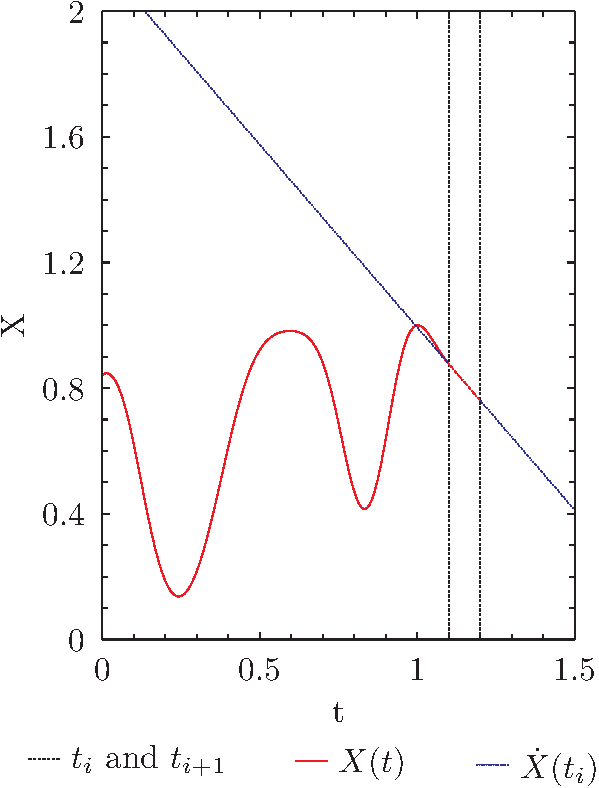
\includegraphics[width=\linewidth]{euler_demo1.pdf}%
}%
\only<7>{%
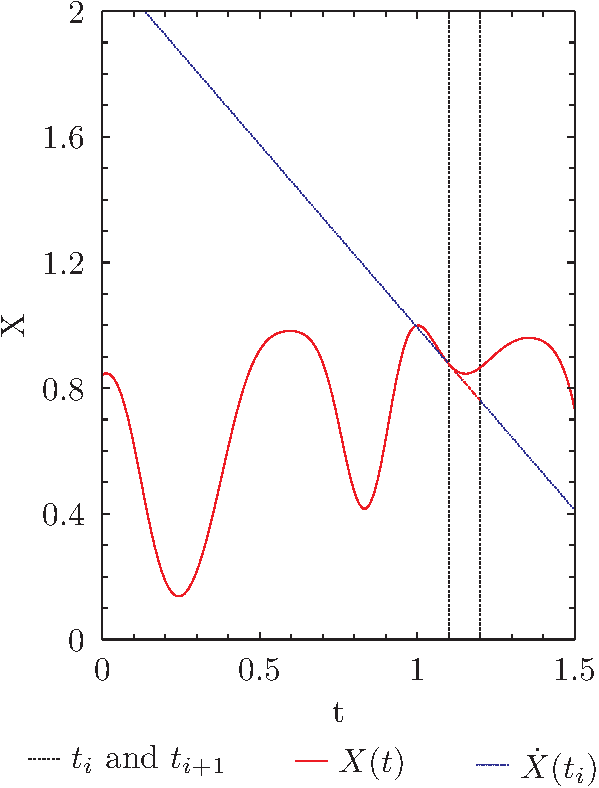
\includegraphics[width=\linewidth]{euler_demo2.pdf}%
}%
\end{column}
\end{columns}
\end{frame}


\begin{frame}
\frametitle{Why does this work? What is the error}
\begin{itemize}
\item<1-> Multiple justifications for why.

\item<2-> First 2 terms in Taylor series {{\color{gray} Zeigler et al.}}:

\begin{equation*}
\mathbf{X}(t_{i+1}) = \mathbf{X}(t_{i})+h f_{ode}(\mathbf{X}(t_i),t_i)+h^2\ldots +\ldots.
\end{equation*}

\item<3-> ``Local truncation error"  $~h^2=h^{p+1}$.

\item<3-> Global error $~h=h^p$.

\item<4-> Convergence, but not uniform.
\end{itemize}
\end{frame}

\begin{frame}
\frametitle{Why does this work? The Runge Kutta family}
\begin{itemize}

\item<1-> In general.

\begin{equation*}
\mathbf{X}(t_{i+1})-\mathbf{X}(t_{i}) = \int_{t_i}^{t_{i+1}} f_{ode}(\mathbf{X}(t_i),t_i) dt \only<2-> = h f_{ode}(\mathbf{X}(\tau),\tau)
\end{equation*}

\item <2-> \textit{Mean Value theorem for integrals} $t_i\leq \tau\leq t_{i+1}$.

\item<3-> Guess $\tau=t_i$.

\item<4-> More generally, (\textit{Explicit} and \textit{single step}), Runge-Kutta family:

\begin{align*}
\mathbf{X}(t_{i+1})-\mathbf{X}(t_{i}) &= \int_{t_i}^{t'} f_{ode}(\mathbf{X}(t_i),t_i) dt + \ldots \int_{t^{(m)}}^{t_{i+1}} f_{ode}(\mathbf{X}(t_i),t_i) dt \only<5->{\\ &= h \sum_{j=1}^{m} c_j f_{ode}(\mathbf{X}(\tau_j),\tau_j)}
\end{align*}

\item<5-> Use $f_{ode}(\mathbf{X}(t_i),t_i)$ to approximate $\mathbf{X}(\tau_1)$ etc.


\item<1-> {\color{gray} L. Zheng, X. Zhang, Modeling and Analysis of Modern Fluid Problems, 2017, chapter 8}:

\end{itemize}
\end{frame}


\begin{frame}
\frametitle{Explicit Runge Kutta methods}
\begin{itemize}

\item<1-> We want:

\begin{equation*}
\mathbf{X}(t_{i+1})-\mathbf{X}(t_{i}) =  h \sum_{j=1}^{m} b_j \mathbf{K}_j
\end{equation*}

\item<1-> With: $\mathbf{K}_1 =  f_{ode}(\mathbf{X}(t_i),t_i)$, $\mathbf{K}_2 =  f_{ode}(\mathbf{X}(t_i)+ha_{21}\mathbf{K}_{1},t_i+c_2h)$ etc.

\item<2-> Want exact to $p$'th order. Can be found with taylor expansion of $\mathbf{X}(t_{i})$.

\item<3-> 2nd order (Heun's method):

\begin{align*}
\mathbf{X}(t_{i+1})-\mathbf{X}(t_{i}) &= \frac{h}{2}(\mathbf{k}_1+\mathbf{k}_2)\\
\mathbf{k}_1 &= f_{ode}(\mathbf{X}(t_i),t_i)\\
\mathbf{k}_2 &= f_{ode}(\mathbf{X}(t_i)+h\mathbf{k}_1,t_i+h)
\end{align*}

\item<1-> {{\color{gray} Martha L. Abell, James P. Braselton, Differential Equations with Mathematica (Fourth Edition), 2016}}:
\end{itemize}
\end{frame}


\subsection{4th order Runge Kutta}


\begin{frame}
\frametitle{The 4th order Runge Kutta method}
\begin{columns}
\begin{column}{0.5\linewidth}
\begin{itemize}

\item<1-> RK4, often simply called the Runge Kutta method:

\begin{align*}
\mathbf{X}(t_{i+1})-\mathbf{X}(t_{i}) &= \frac{h}{6}(\mathbf{k}_1+2\mathbf{k}_2+2\mathbf{k}_3+\mathbf{k}_4 )\\
\mathbf{k}_1 &= f_{ode}(\mathbf{X}(t_i),t_i)\\
\mathbf{k}_2 &= f_{ode}(\mathbf{X}(t_i)+\frac{h}{2}\mathbf{k}_1,t_i+\frac{h}{2})\\
\mathbf{k}_3 &= f_{ode}(\mathbf{X}(t_i)+\frac{h}{2}\mathbf{k}_2,t_i+\frac{h}{2})\\
\mathbf{k}_4 &= f_{ode}(\mathbf{X}(t_i)+h\mathbf{k}_3,t_i+h)\\
\end{align*}

\item<2-> Almost default in \lstinline{scipy.integrate.solve_ivp} and matlab \lstinline{ode45}.

\end{itemize}
\end{column}
\begin{column}{0.5\linewidth}
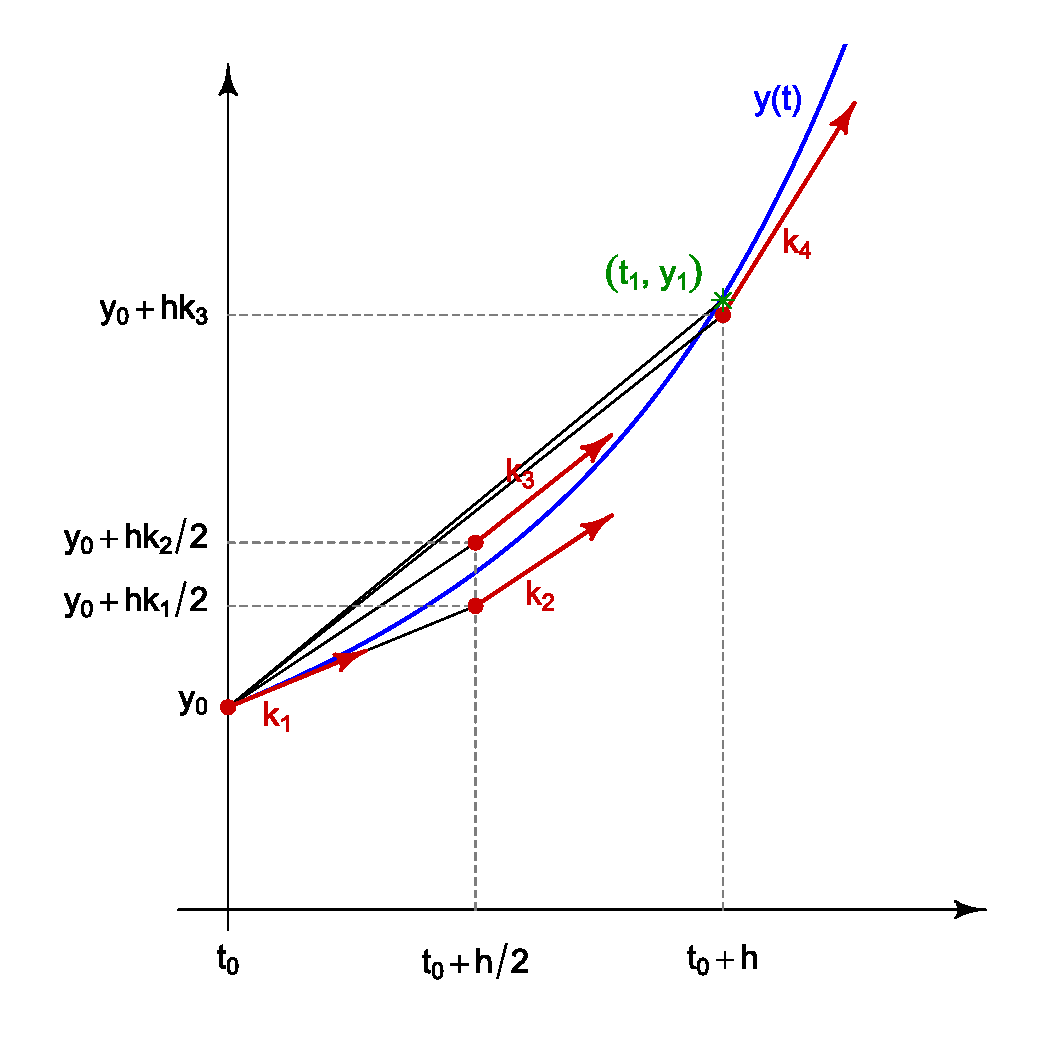
\includegraphics[width=\linewidth]{Runge-Kutta_slopes.pdf}

{\color{gray} Wikipedia-user HilberTraum, published under creative commins: CC BY-SA 4.0}
\end{column}
\end{columns}
\end{frame}

\begin{frame}
\frametitle{The General explicit Runge Kutta method}
\begin{itemize}

\item<1-> General explicit, single step, fixed size, Runge Kutta method

\begin{align*}
\mathbf{X}(t_{i+1})-\mathbf{X}(t_{i}) &=  h \sum_{j=1}^{m} b_j \mathbf{K}_j\\
\mathbf{k}_1 &= f_{ode}(\mathbf{X}(t_i),t_i)\\
\mathbf{k}_2 &= f_{ode}(\mathbf{X}(t_i)+ha_{21} \mathbf{k}_1,t_i+c_2 h)\\
\mathbf{k}_3 &= f_{ode}(\mathbf{X}(t_i)+ha_{31} \mathbf{k}_1+ha_{32} \mathbf{k}_2,t_i+c_3 h)
&\vdots
\end{align*}

\item<2-> Expressed in Butcher tableu:

\begin{tabular}{l | @{\quad} c @{\quad} c @{\quad} c}
$c_1=0$ \\
$c_2$ & $a_{21}$\\
$c_3$ & $a_{31}$ &  $a_{32}$\\
$c_n$ & $a_{n1}$ &  $a_{n2}$ & $\hdots$\\
\midrule
& $b_1$ & $b_2$ & $\hdots$
\end{tabular}


\end{itemize}
\end{frame}


\begin{frame}[fragile]
\frametitle{Euler Implementations}
\begin{lstlisting}
state_type Data = Data0;
state_type dDatadt;
size_t time_res = T/timestep;
for (size_t i = 1; i < time_res; ++i)
{
    double t=i*dt;
    ODE(Data,dDatadt,t);
    //Euler time evolution
    //Data +=timestep*dDatadt; 1 variable
    for (uint i = 0; i<Data.size(); ++i)
        Data[i]+=timestep*dDatadt[i];
    save_step( Data , i*timestep );
};
\end{lstlisting}
\end{frame}





\begin{frame}[fragile]
\frametitle{RK4 Implementations (1/2)}
\begin{lstlisting}
state_type Data = Data0;
state_type temp=Data0;
state_type K1,K2,K3,K4;
size_t time_res = T/timestep;
for (size_t i = 1; i < time_res; ++i)
{
    double t=i*timestep;
    //substep 1
    ODE(Data,K1,t);
    for (uint i = 0; i<Data.size(); ++i)
        temp[i]=Data[i]+timestep*K1[i]/2;
    //substep 2
    ODE(Data,K2,t+timestep/2);
    for (uint i = 0; i<Data.size(); ++i)
        temp[i]=Data[i]+timestep*K2[i]/2;
\end{lstlisting}
\end{frame}

\begin{frame}[fragile]
\frametitle{RK4 Implementations (2/2)}
\begin{lstlisting}
    //substep 3
    ODE(Data,K3,t+timestep/2);
    for (uint i = 0; i<Data.size(); ++i)
        temp[i]=Data[i]+timestep*K3[i];
    //substep 4
    ODE(temp,K4,t+timestep);
    //Read data
    for (uint i = 0; i<Data.size(); ++i)
        Data[i]+=timestep*(K1[i]+2.0*K2[i]+2.0*K3[i]+K4[i])/6.0;
    save_step( Data , i*timestep );
}
\end{lstlisting}
\end{frame}


\begin{frame}[fragile]
\frametitle{``Correct" way}
\begin{lstlisting}
#include <boost/array.hpp>
#include <boost/numeric/odeint.hpp>
using namespace boost::numeric::odeint;
typedef boost::array< double, 6 > state_type;
...
size_t steps = integrate_const(
    runge_kutta4< state_type >(),
    ODE,   //Lorentz-force
    Data0 ,//{pos0,v0}
    0.0 ,  //t0=0
    T ,    //max time
    timestep ,//length of each step
    save_step //User defined save data function
);
\end{lstlisting}
\end{frame}



\section{Testing the methods [5 MIN]}

\begin{frame}
\frametitle{Does it work}
\begin{itemize}

\item<1-> Test, same proton in a solenoid use $\theta=\ang{60}$ reference, had:

\begin{equation*}
R \approx \SI{0.5}{\meter}\sin(\theta)\approx \SI{0.45}{\meter} \quad T=\frac{2\pi}{\omega_c} \approx \SI{10}{\micro\second}
\end{equation*}

\item<2-> Compare Analytic, Euler, Runge-Kutta 4.

\item<3-> Consider $\theta=\ang{60}$, $h=\SI{0.01}{\micro\second}$, $h=\SI{0.1}{\micro\second}$ and  $h=\SI{0.1}{\micro\second}$.

\item<4-> Check error on $|\vec{v}|$, $R=\sqrt{y^2+z^2}$ and $x(t)$.
\end{itemize}
\end{frame}


\makeatletter
\begin{frame}
\frametitle{At a glance, 3D view}
    \global\beamer@shrinktrue
    \gdef\beamer@shrinkframebox{
        \setbox\beamer@framebox=\vbox to\beamer@frametextheight{
            \centering
            $h=t_{i+1}-t_i=\SI{0.01}{\micro\second}$

            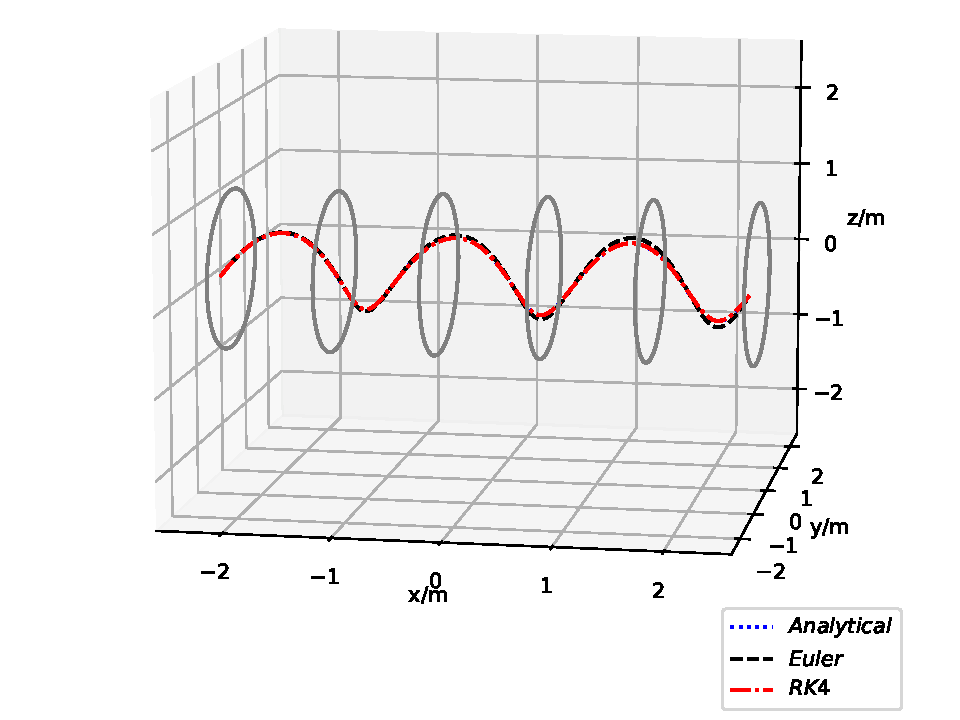
\includegraphics[height=0.9\beamer@frametextheight]{Solenoid_compare001_3D.pdf}

            3129 steps
        }
    }
\end{frame}
\makeatother

\makeatletter
\begin{frame}
\frametitle{At a glance, 3D view}
    \global\beamer@shrinktrue
    \gdef\beamer@shrinkframebox{
        \setbox\beamer@framebox=\vbox to\beamer@frametextheight{
            \centering
            $h=t_{i+1}-t_i=\SI{0.1}{\micro\second}$

            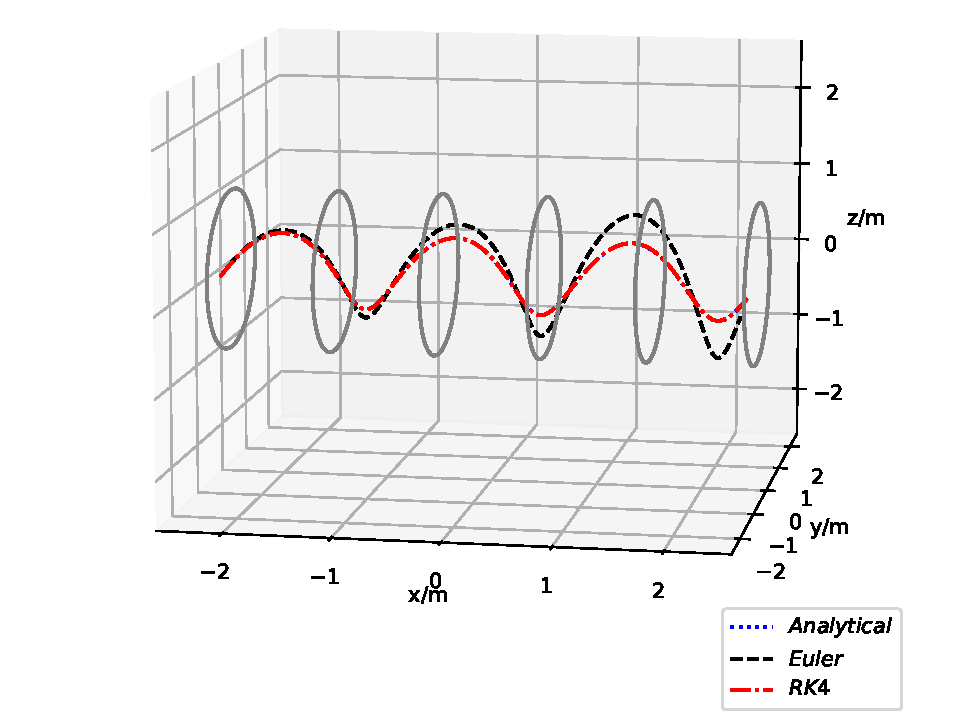
\includegraphics[height=0.9\beamer@frametextheight]{Solenoid_compare01_3D.pdf}

            312 steps
        }
    }
\end{frame}
\makeatother

\makeatletter
\begin{frame}
\frametitle{At a glance, 3D view}
    \global\beamer@shrinktrue
    \gdef\beamer@shrinkframebox{
        \setbox\beamer@framebox=\vbox to\beamer@frametextheight{
            \centering
            $h=t_{i+1}-t_i=\SI{1.0}{\micro\second}$

            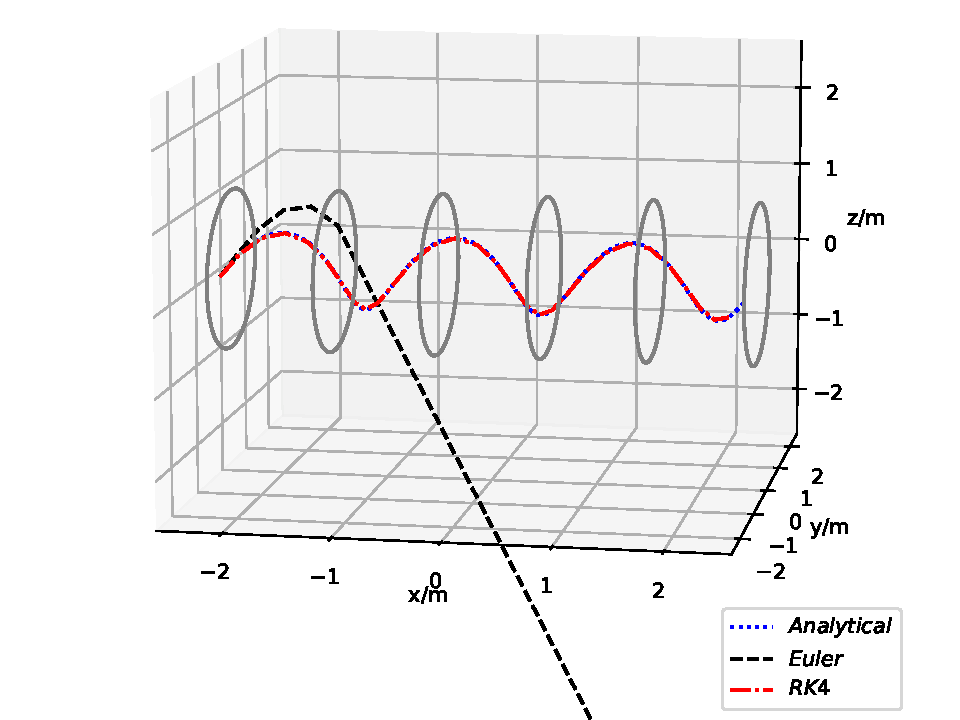
\includegraphics[height=0.9\beamer@frametextheight]{Solenoid_compare1_3D.pdf}

            31 steps.
        }
    }
\end{frame}
\makeatother

\begin{frame}
\frametitle{At a glance, front view, no border}
\only<1>{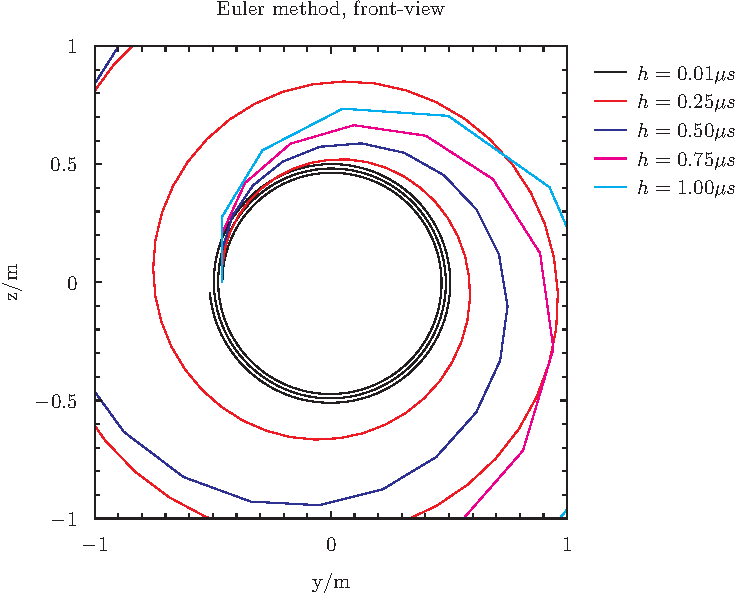
\includegraphics[width=\linewidth]{solenoid_euler_yz_view.pdf}}%
\only<2>{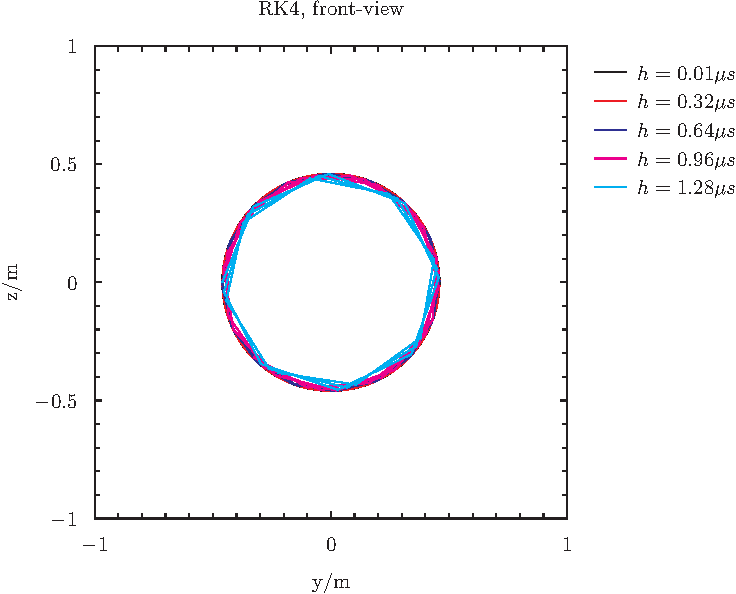
\includegraphics[width=\linewidth]{solenoid_RK_yz_view.pdf}}
\end{frame}

\begin{frame}
\frametitle{Constant radius?}
\only<1>{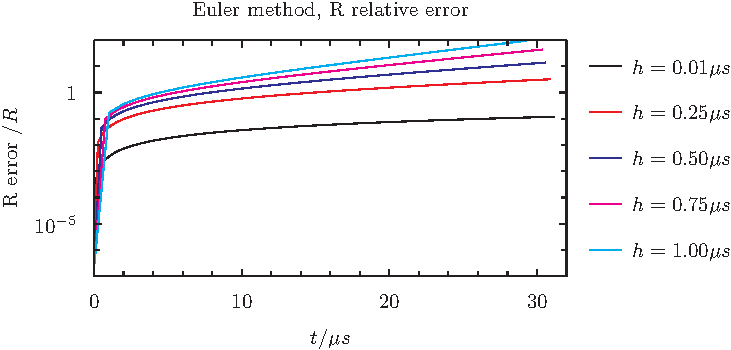
\includegraphics[width=\linewidth]{solenoid_euler_Rt.pdf}}%
\only<2>{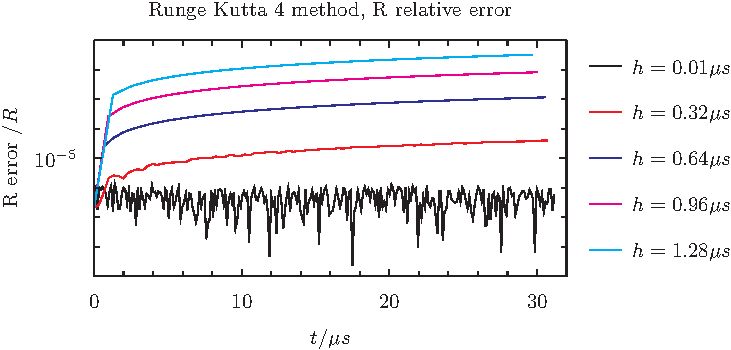
\includegraphics[width=\linewidth]{solenoid_RK4_Rt.pdf}}
\end{frame}


\begin{frame}
\frametitle{Constant speed?}
\only<1>{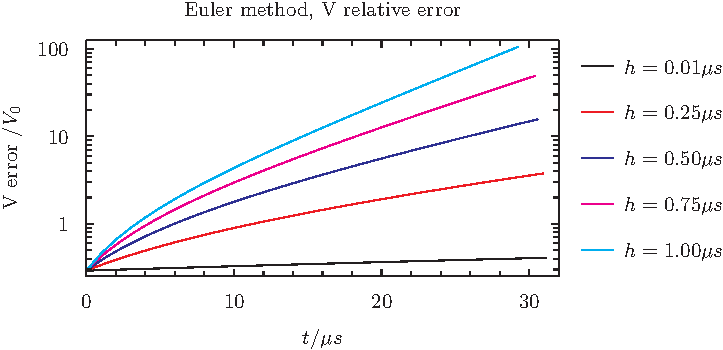
\includegraphics[width=\linewidth]{solenoid_euler_Vt.pdf}}%
\only<2>{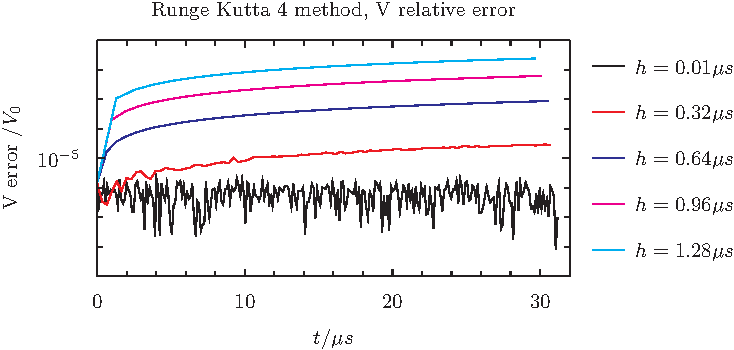
\includegraphics[width=\linewidth]{solenoid_RK4_Vt.pdf}}
\end{frame}

\begin{frame}
\frametitle{Error as function of $h$}
\only<1>{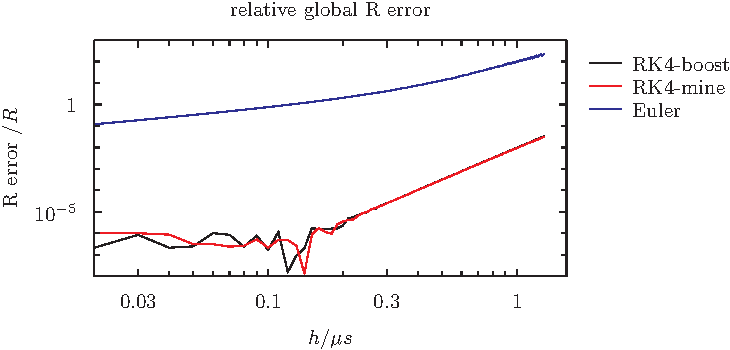
\includegraphics[width=\linewidth]{solenoid_Rh.pdf}}%
\end{frame}

\section{Introducing Adaptive step size [5 MIN]}


\begin{frame}
\frametitle{Adaptive step size, why}



\begin{columns}
\begin{column}{0.5\linewidth}
\begin{itemize}
\item <1-> $h$ must be small ``enough"

\item <2-> Hard to pick, and may change:

\item <3-> Inhomogeneous fields (here Earth magnetic field)

\item <4-> time dependent fields (here the cyclotron)

\item <5-> Let the computer pick $h$.

\end{itemize}
\end{column}
\begin{column}{0.5\linewidth}


\only<3>{%
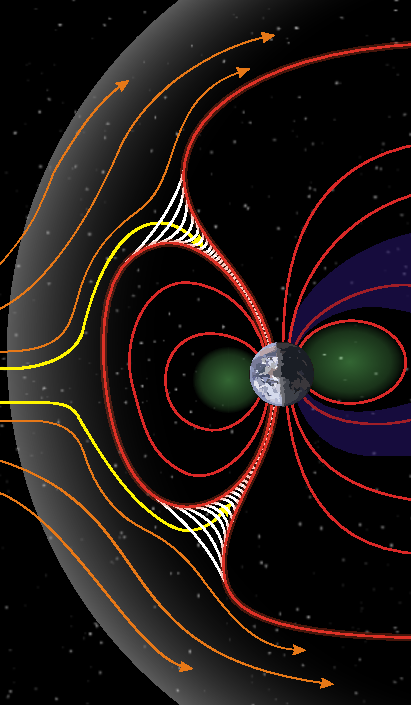
\includegraphics[width=0.8\linewidth]{Structure_of_the_magnetosphere_Nasa.pdf}%

{\color{gray} Illustration originally from Nasa. Published on wikipedia, in Public Domain (Cropped to fit page) }
}%


\only<4>{%
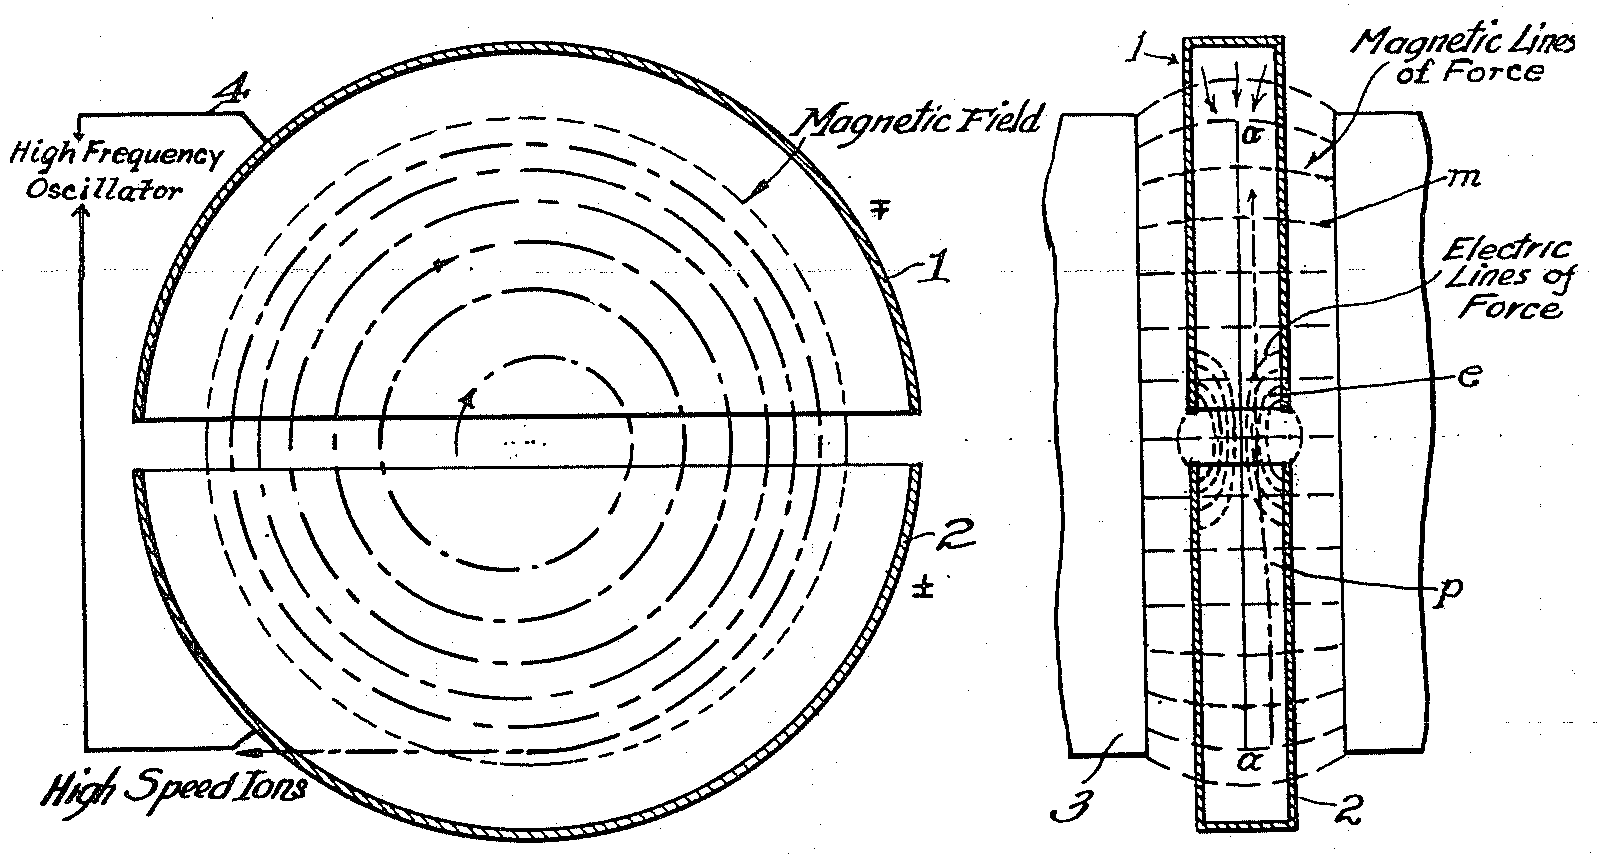
\includegraphics[width=\linewidth]{ Cyclotron_patent.png}

{\color{gray} Ernest O. Lawrence, 1934, U.S. Patent 1,948,384; image in Public Domain.}
}%

\end{column}
\end{columns}
\end{frame}


\begin{frame}
\frametitle{Runge-Kutta Adaptive step size, how}
\begin{itemize}
\item <1-> Reduce $h$ until the ``error" is small enough

\item <2-> Use 2 different methods, $\mathbf{x}(t_{i+1})$, $\mathbf{x}'(t_{i+1})$.

\item <3-> Approximate ``Error" as  $|\mathbf{x}(t_{i+1})-\mathbf{x}'(t_{i+1})|$.

\item <4-> Most often order 4 and 5 with same $\mathbf{k}_i$.
\end{itemize}
\end{frame}

\begin{frame}
\frametitle{Runge-Kutta Dormund Prince 4-5, }

\begin{itemize}


\item <1->\lstinline{ode45} in Matlab , \lstinline{RungeKutta_dopri5} in \lstinline{boost::odeint}.
\begin{align*}
\mathbf{X}(t_{i+1})-\mathbf{X}(t_{i}) &=  h \sum_{j=1}^{m} b_j \mathbf{k}_j\\
\mathbf{X}(t_{i+1})-\mathbf{X}(t_{i}) &=  h \sum_{j=1}^{m} b_j' \mathbf{k}_j
\end{align*}

\begin{align*}
\mathbf{X}(t_{i+1})-\mathbf{X}(t_{i}) &=  h \sum_{j=1}^{m} b_j \mathbf{K}_j\\
\mathbf{k}_i &= f_{ode}(\mathbf{X}(t_i)+h \sum_j^{i-1} a_{ki} \mathbf{k}_i+ha_{32},t_i+c_3 h)
&\vdots
\end{align*}

\item<2-> 4th and 5th order, hence ode 45. Keeps 5th order term if error less than absolute and relative threshold.

{\color{gray} Dormand, J. R.; Prince, P. J. (1980), "A family of embedded Runge-Kutta formulae", Journal of Computational and Applied Mathematics}
\end{itemize}
\end{frame}


\begin{frame}
\frametitle{Butcher Tableu of Dormund Prince 4/5}
\begin{tabular}{c | @{\quad} c @{\quad} c @{\quad} c @{\quad} c @{\quad} c @{\quad} c @{\quad} c @{\quad} c}
$c_i$ & $a_{ij}$ & $\hdots$\\
\midrule
$0$ \\
$\frac{1}{5}$ & $\frac{1}{5}$\\
$\frac{3}{10}$ & $\frac{3}{40}$ &  $\frac{9}{40}$\\
$\frac{4}{5}$ & $\frac{40}{45}$ &  $-\frac{56}{15}$  &  $-\frac{32}{9}$\\
$\frac{8}{9}$ & $\frac{19372}{6561}$ & $−\frac{25360}{2187}$ & $\frac{64448}{6561}$ & $−\frac{212}{729}$\\
$1$ & $\frac{9017}{3168}$ & $-\frac{355}{33}$ & $\frac{46732}{5247}$ & $\frac{49}{176}$  & $-\frac{5103}{18656}$\\
$1$ & $\frac{35}{384}$  & $0$	 & $\frac{500}{1113}$ & $\frac{125}{192}$ & $-\frac{2187}{6784}$ & $\frac{11}{84}$\\
\midrule
$/b$  & $\frac{35}{384}$ & $0$ & $\frac{500}{1113}$ & $\frac{125}{192}$ & $-\frac{2187}{6784}$ & $\frac{11}{84}$ & $0$\\
$/b'$ & $\frac{5179}{57600}$ & $0$ & $\frac{7571}{16695}$ & & $\frac{393}{640}$ & $-\frac{92097}{339200}$& $\frac{187}{2100}$ & $\frac{1}{40}$\\
\end{tabular}
\end{frame}

\begin{frame}[fragile]
\frametitle{Testing adaptive step-size}
\begin{lstlisting}
#include <boost/array.hpp>
#include <boost/numeric/odeint.hpp>
using namespace boost::numeric::odeint;
typedef boost::array< double, 6 > state_type;
...
size_t steps = integrate_adaptive(
    runge_kutta_dopri5< state_type >(),
    ODE,   //Lorentz-force
    Data0 ,//{pos0,v0}
    0.0 ,  //t0=0
    T ,    //max time
    timestep ,//length of each step (initial)
    save_step //User defined save data function
);
\end{lstlisting}
\end{frame}

\begin{frame}[fragile]
\frametitle{Testing adaptive step-size}
\begin{lstlisting}
#include <boost/array.hpp>
#include <boost/numeric/odeint.hpp>
using namespace boost::numeric::odeint;
typedef boost::array< double, 6 > state_type;
...
size_t steps = integrate_adaptive(
    make_controled( absErr, relErr , runge_kutta_dopri5< state_type >() ),
    ODE,   //Lorentz-force
    Data0 ,//{pos0,v0}
    0.0 ,  //t0=0
    T ,    //max time
    timestep ,//length of each step (initial)
    save_step //User defined save data function
);
\end{lstlisting}
\end{frame}

\begin{frame}[fragile]
\frametitle{Testing adaptive step-size}
\begin{lstlisting}
#include <boost/array.hpp>
#include <boost/numeric/odeint.hpp>
using namespace boost::numeric::odeint;
typedef boost::array< double, 6 > state_type;
...
size_t steps = integrate(
    ODE,   //Lorentz-force
    Data0 ,//{pos0,v0}
    0.0 ,  //t0=0
    T ,    //max time
    timestep ,//length of each step (initial)
    save_step //User defined save data function
);
\end{lstlisting}
\end{frame}

\begin{frame}
\frametitle{Example, cyclotron}
\begin{columns}
\begin{column}{0.5\linewidth}
\begin{itemize}
\item<1-> Electric field accelerates, magnetic contains.

\item<2-> Single gab, oscillating field.

\item<3-> Uses Cyclotron frequency

\item<4-> Analytical final speed, in principle path.

\begin{equation*}
\frac{R|q|B}{m} = v_\perp
\end{equation*}

\end{itemize}
\end{column}
\begin{column}{0.5\linewidth}
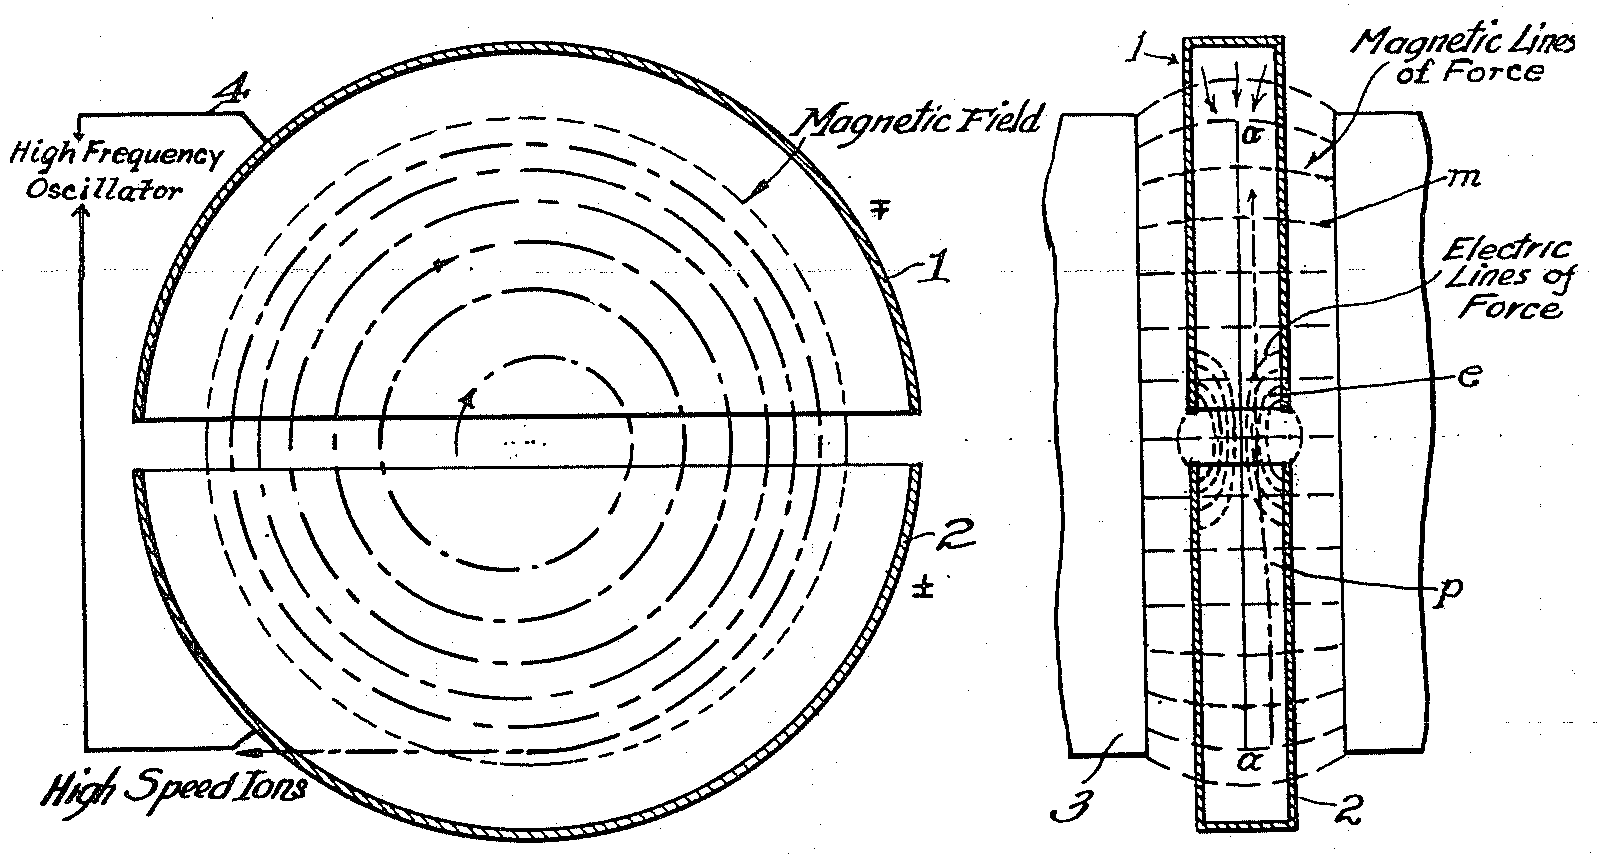
\includegraphics[width=\linewidth]{ Cyclotron_patent.png}
{\color{gray} Ernest O. Lawrence, 1934, U.S. Patent 1,948,384; image in Public Domain.}
\end{column}
\end{columns}
\end{frame}

\subsection{When adaptive step-size fails}

\begin{frame}[fragile]
\frametitle{Naive setup}
\begin{lstlisting}
size_t steps = integrate(
//Default to adaptive- Dopri5, this is fine
    ODE      , //Lorentz-force
    Data0    , //{pos0,v0}
    0.0      , //t0=0
    T        , //Here 500 micro second
    timestep , //Here 0.1 (intentionally too large)
    save_step);//User defined save data function
\end{lstlisting}
\end{frame}

\begin{frame}
\frametitle{Does it help/work}
\begin{columns}
\begin{column}{0.5\linewidth}
\begin{itemize}
\item<1-> With fixed step size (Same method, accept all) 4999 points

\item<2-> Trust default setup:

\item<2-> Epic fail Why?


\end{itemize}
\end{column}
\begin{column}{0.5\linewidth}
\only<1>{%
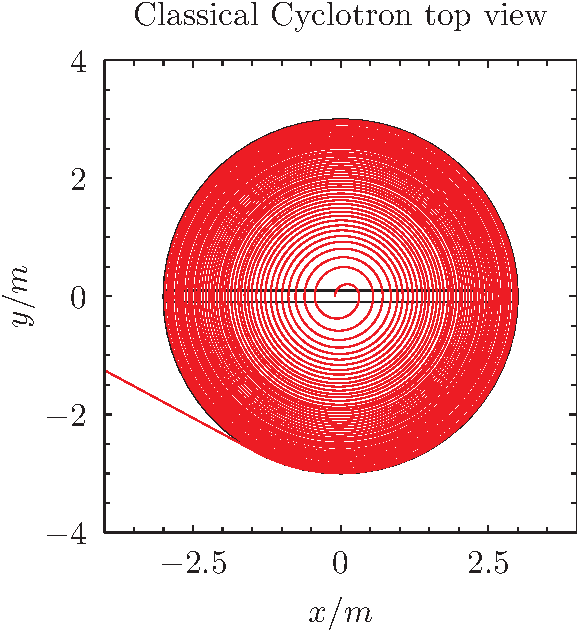
\includegraphics[width=\linewidth]{ cyclotron_noadapt_xy-view.pdf}%

4999 points!}%
\only<2->{%
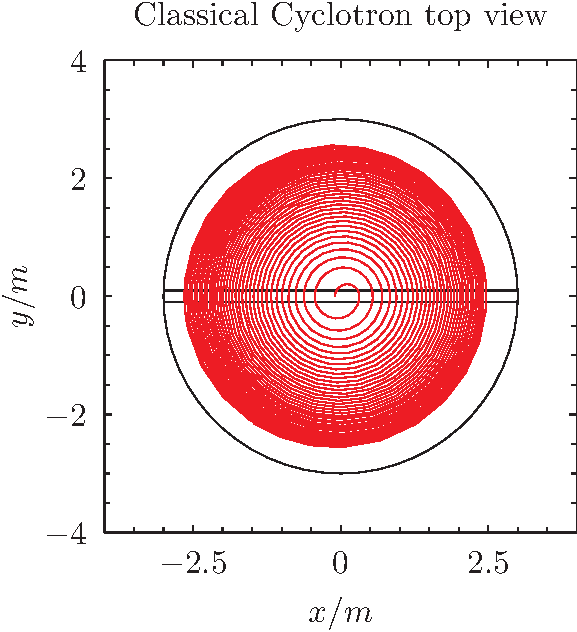
\includegraphics[width=\linewidth]{ cyclotron_badadapt_xy-view.pdf}%

2070 points}%


\end{column}
\end{columns}

\end{frame}


\begin{frame}
\begin{center}
\only<1>{%
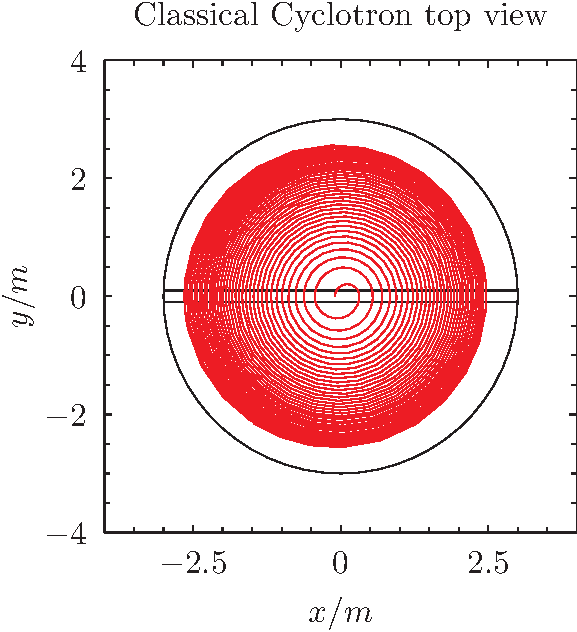
\includegraphics[width=0.7\linewidth]{ cyclotron_badadapt_xy-view.pdf}%

Default choice,  2070 points.
}%
\only<2->{%
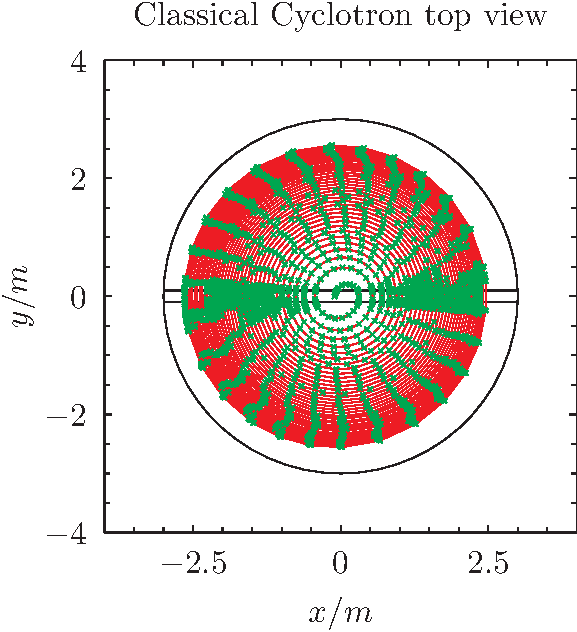
\includegraphics[width=0.7\linewidth]{ cyclotron_badadapt_xy1-view.pdf}%

Default choice,  2070 points.
}%
\only<3->{%
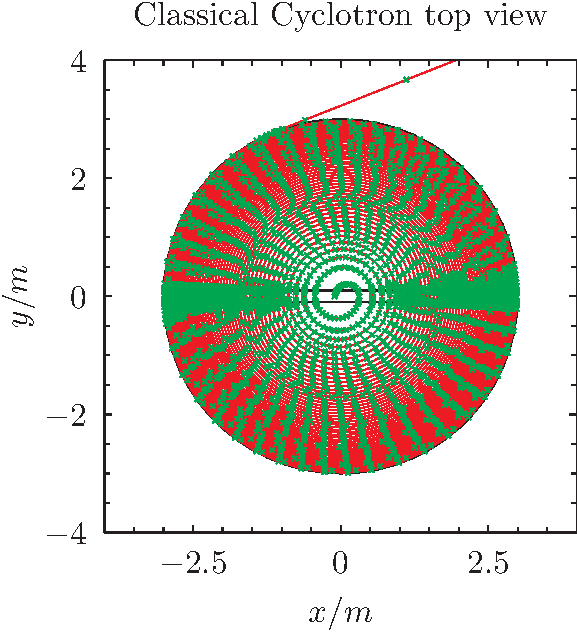
\includegraphics[width=0.7\linewidth]{ cyclotron_badadapt_xy2-view.pdf}%

\lstinline{make_controlled( 1E-7 , 1E-7 , runge_kutta_dopri5< state_type >() )},  3714 points.
}%
\only<4->{%
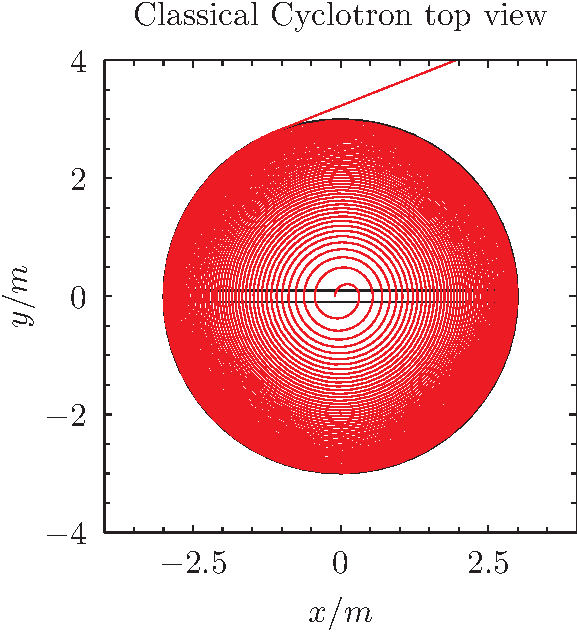
\includegraphics[width=0.7\linewidth]{ cyclotron_badadapt_xy3-view.pdf}%

\lstinline{make_controlled( 1E-7 , 1E-7 , runge_kutta_dopri5< state_type >() )},  3714 points.
}%
\only<5->{%
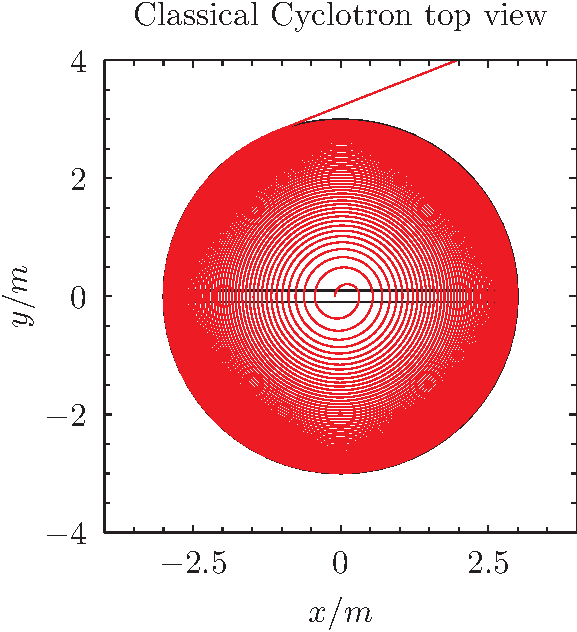
\includegraphics[width=0.7\linewidth]{ cyclotron_badadapt_xy4-view.pdf}%

\lstinline{make_controlled( 1E-12 , 1E-12 , runge_kutta_dopri5< state_type >() )},  23850 points.
}%
\end{center}
\end{frame}

\begin{frame}
\frametitle{Analytic agreement}
...
\end{frame}


\section{Non-analytical systems: Toroidal coils and dipoles [10 MIN]}

\begin{frame}
\frametitle{Non-analytic systems}
\end{frame}

\section{Conclusion and question}

\begin{frame}
\frametitle{Questions}
\end{frame}


%Electric and magnetic fields
%The Lorentz force
%Newtons 2nd law, ordinary differential equation
%Alternative, electric and magnetic potentials

\end{document}
